% ============================================================
% v2/sections/methods.tex  モデルと実験方法（短縮・再構成版 2026-10-27）
% 数字は sections/methods.tex（第2弾の照合済み）と Claude Code の報告から。
% ============================================================
\section{モデルと実験方法}\label{sec:method}

\begin{figure}[tbp]
  \centering
  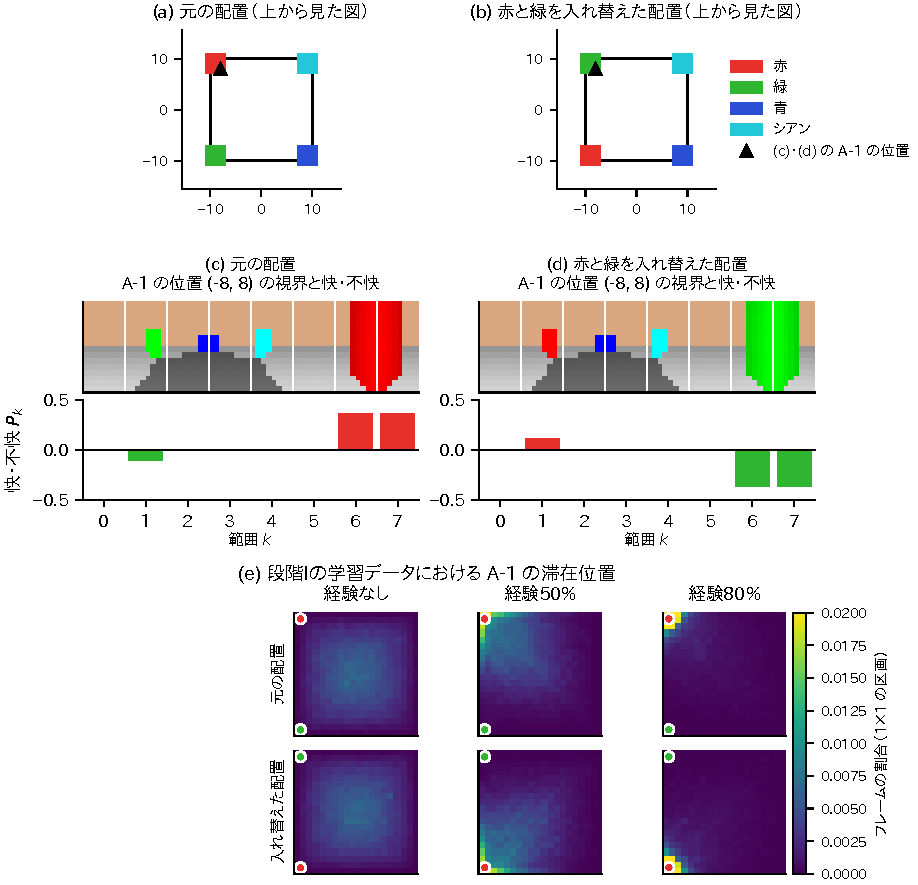
\includegraphics[width=0.49\linewidth]{figs/env_conditions}\hfill
  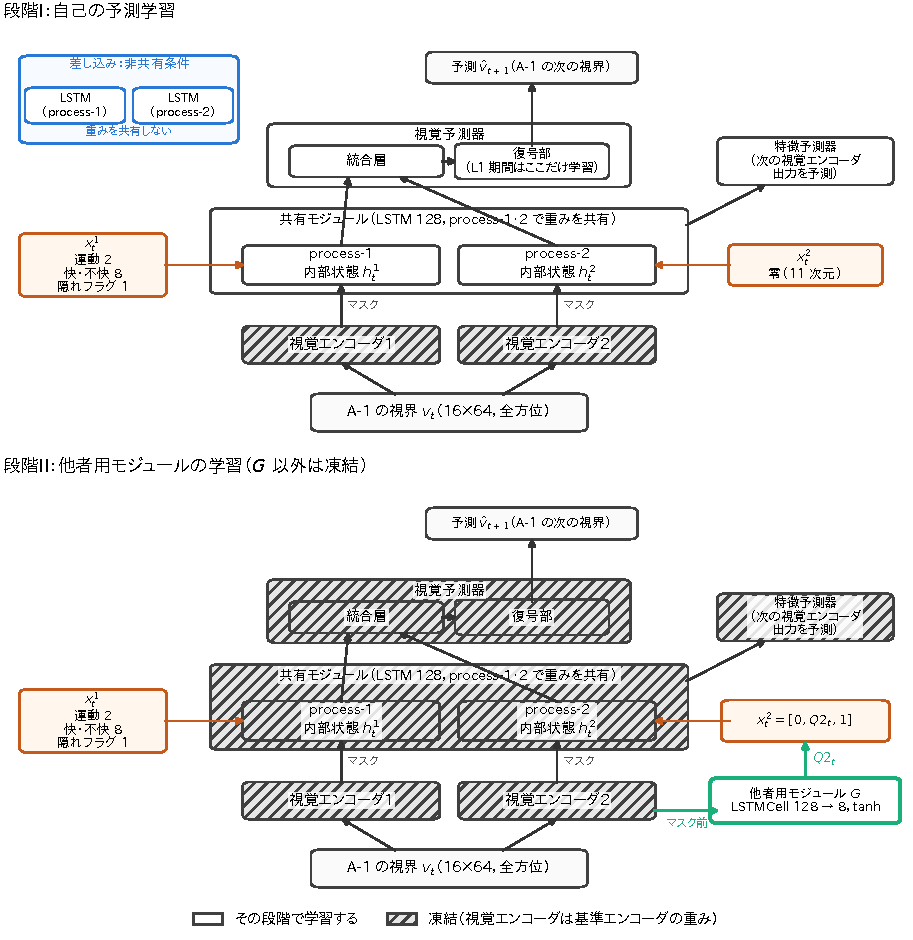
\includegraphics[width=0.49\linewidth]{figs/network}
  % 左：環境と条件（env_conditions.pdf）。右：ネットワークと2段階の学習（network.pdf）。
  % 投稿の前に一枚の図に作り直すことを検討（Claude Code）。
  \caption{環境とモデル．左：アリーナと赤・緑を入れ替えた配置，全方位の視界と方向ごとの快・不快 $P_k$，段階Iの学習データにおける A-1 の滞在位置．右：ネットワーク．視覚エンコーダ1・2（斜線，凍結）が A-1 の視界を読み，重みを共有した LSTM の process-1（自分）と process-2（他者）が別々の内部状態 $h^1$，$h^2$ を持つ．差し込みは非共有条件で分ける部分．}
  \label{fig:model}
\end{figure}

\subsection{環境と価値の信号}\label{sec:env}
環境は文献\cite{noguchi2022superposition}と同じ $20\times20$ のアリーナで，四隅の外に赤・緑・青・シアンの立方体を置いた（図\ref{fig:model}）．
エージェントは2体で，学習するのは A-1 だけである．
A-1 は回転しない全方位カメラで $16\times64$ 画素の視界 $v_t$ を得る．
文献\cite{noguchi2022superposition}との違いとして，エピソードごとに確率 1/2 で赤と緑の位置を入れ替えた．
入れ替えのない環境では，「赤の方へ動く」ことと「特定の場所へ動く」ことが区別できないためである．
各エピソードは 101 フレームで，A-1 は1ステップに1の距離を動くか，休止（確率 0.005 で始まり 10〜30 ステップ）する．

A-1 の価値は，視界から毎ステップ計算する8次元の快・不快 $P_t$ として与えた．
カメラの8列ごとの範囲 $k$ で $P_{t,k}=(n^{\mathrm{like}}_{t,k}-n^{\mathrm{dislike}}_{t,k})/128$ とし，好きな色を赤，嫌いな色を緑とした（$n$ は各色の画素数）．
値が0以外になるのは範囲 0・1・6・7 だけである．
この値は人が与える信号であり，ネットワークが学ぶのは，この信号と自分の行動・視界の変化との関係である．

価値に従う一歩は，視界の中の赤の円周上の重心の方角へ進む規則で作った（壁では沿って進み，進めないときはランダム）．
A-1 は休止していない各ステップで，確率 $p$ で規則の一歩を，残りでランダムな一歩をとる．
$p=0$ を経験なし条件，$p=0.5$ を経験50\%条件，$p=0.8$ を経験80\%条件と呼ぶ．
$p$ は規則の一歩を選ぶ確率で，実際に規則で動いた一歩の割合は経験50\%条件で 48\%，経験80\%条件で 57\% であった．
乱数は，同じエピソード番号で配置・初期位置・休止の時刻が条件の間で一致するように設定した．
ただし $p$ を上げると位置の分布も変わり，赤から距離5以内にいるフレームの割合は約 0.03，約 0.33，約 0.85 であった．
この交絡を扱うため，後述の符号無作為条件を作った．

段階Iでは A-2 は静止し，各条件で学習用 3000・評価用 300 エピソードを集めた．
段階IIの学習と，他者側の評価のうち符号に従う分・真値条件・照合では，A-1 はランダムに歩き，A-2 は自分の視界で同じ規則を用いて一歩ごとに確率 0.5 で好きな色へ向かう．
A-2 が常に緑を好むデータ（緑好みデータ）と，エピソードごとに緑好き・赤好きが変わるデータ（好み混合データ）を用いた．

\subsection{ネットワーク}\label{sec:network}
ネットワークは文献\cite{noguchi2022superposition}に従う（図\ref{fig:model}）．
二つの視覚エンコーダが A-1 の視界を読み，共有モジュール（128 ユニットの LSTM）が process-1 と process-2 で重みを共有して内部状態 $h^1_t$，$h^2_t$ を別々に持つ．
視覚予測器が両者をまとめて A-1 自身の次の視界 $v_{t+1}$ を予測し，特徴予測器が $h^1$，$h^2$ から次の視覚エンコーダの出力を予測する．
学習中は視覚を各ステップ確率 0.99 で隠す．
文献\cite{noguchi2022superposition}では process-1 の入力は運動 $m_t$ だったが，本研究では $x^1_t=[m_t,P_t,b_t]$（11次元）とした．
運動は 5〜15 ステップの区間を交互に置いて隠し（$t\ge1$ の約48\%），隠れた区間では $m_t=0$，隠れフラグ $b_t=1$ とし，$P_t$ を区間の最初の値に保つ．
運動が分からないときに次の視界を当てるには自分の動きを推し量る必要があり，価値に従って動いた経験があれば「快の高い方へ動いた」と推し量る理由が生まれる．
段階Iでは process-2 の入力は零である．

視覚エンコーダは，文献\cite{noguchi2022superposition}の設定（運動を入力，入れ替えなし）で再現学習した重み（基準エンコーダ）に，すべての条件で固定した．
基準エンコーダを用いた再現モデルでは，$h^1$ から A-1 の位置が $R^2=0.967$，$h^2$ から A-2 の位置が 0.993 で読め，視覚エンコーダ2と1の符号のコサイン類似度（自他一致度）は 0.80 である．
運動以外の入力を加えてエンコーダごと学習すると自他一致度が 0.18〜0.27 にとどまったため，固定した（補足資料）．
したがって自他を同じ符号で表す性質は学んだものではなく与えたものである．

段階Iは，200 エポックの二乗誤差（MSE 期間）で共有モジュール・視覚予測器・特徴予測器を学習し，続く 200 エポックの絶対誤差（L1 期間）で視覚予測器の復号部だけを学習した（AdamW，学習率 $10^{-3}$，重み減衰 0.01，バッチ 10）．
段階IIでは，文献\cite{noguchi2022superposition}の Motion Generator と同じ構成の他者用モジュール $G$ を加え，マスク前の視覚エンコーダ2の出力から8次元の $Q2_t$ を作って process-2 の快・不快の枠に入れ（$x^2_t=[0,Q2_t,1]$），$G$ 以外を凍結して予測誤差で学習した．

\subsection{条件と対照}\label{sec:conditions}
条件と組の一覧，各指標の位置づけを表\ref{tab:design}に示す．
同じシードで学習した各条件のモデルを一つの「組」とし，同じ組の中では初期値・バッチの順・運動を隠す区間を一致させた．
事前登録した判定は本番の3組（組1〜3）で行い，予備の組4と追加の組5・6 も除外せずに報告する．

\paragraph{非共有条件}共有モジュールの LSTM を process-1 用と process-2 用に分け，経験80\%条件のデータで学習した（組1〜3）．process-2 の快・不快を受ける入力の重みは一度も学習されないので，他者側の働きが出ないことは構成からほぼ予想される．

\paragraph{符号無作為条件}経験80\%条件と全く同じ軌跡のデータで，$P_t$ の符号だけをエピソードごとに確率 1/2 で反転した（組1〜3．反転は学習用 3000 のうち 1471 エピソードで，配置とは独立）．位置・運動・視界の系列は経験80\%条件と同じで，価値の信号と行動の対応だけが壊れる．ただし赤へ近づくという行動の履歴そのものは変わらない．

\paragraph{写しの比較}学習を終えた非共有条件のモデルの process-2 用の LSTM に，process-1 用の LSTM の重みを写した．すべて写す場合と，入力の重みのうち快・不快を受ける8列だけを写す場合を作り，経験なし条件の非共有モデルにも同じように写した（組1〜3）．

\paragraph{他者の規則の確率}段階IIの評価用データと同じ作りで，A-2 が確率 0.8 で好きな色へ向かうデータを作った（A-1 の歩き・休止・配置・好きな色は元と全エピソードで一致）．

\begin{table}[tbp]
  \centering
  \footnotesize
  \caption{条件，指標，事前登録の区別}
  \label{tab:design}
  % 仮のファイル：Claude Code が本物の表で上書きする（tables/conditions.tex と metrics.tex を一枚にまとめる）。
\fbox{\parbox{0.9\linewidth}{\centering\ttfamily 表未作成：tables/v2\_design}}

  % 表1（新しく作る，Claude Code）：上段に条件（経験なし・50%・80%，非共有，符号無作為，写し）と組の数，
  % 下段に指標（G3，d_P，G5b，符号に従う分，真値条件の Δ，照合の BA，T2・T5）と位置づけ
  % （事前登録した主／事後に定義／事前登録外）。今の tables/conditions.tex と metrics.tex を一枚にまとめる。
\end{table}

\subsection{測る量}\label{sec:evaluation}
\paragraph{自分側の見込み}運動と視覚を $t=20$ から15ステップ隠し，快・不快を $t=20$ の値に保つ．各ステップの予測を「$t=20$ の位置から色 $X$ の方へ $d$ 歩動いた視界」と比べて最もよく合う $d$ を求め，その傾き $s_X$ から $g=s_{\text{赤}}-\frac13(s_{\text{緑}}+s_{\text{青}}+s_{\text{シアン}})$ を求めた（G3）．運動が分からないときに予測が赤の方へだけ進み続ければ $g>0$ になる．快・不快の符号を反転して保った場合の $g$ も求め，$d_P=(g_{\text{保つ}}-g_{\text{反転}})/2$ を自分側の見込みの快・不快への依存とした．

\paragraph{他者側への働き}主の指標（事前登録）は G5b である．A-2 が静止した評価で，$t=20$〜29 に process-2 の一つの範囲 $k$ だけへ $\pm a$（$a=0.28$）を入れ，10ステップ後の予測画像の中の A-2 の位置のずれの差 $\Delta_k(+a)-\Delta_k(-a)$ を範囲 $k$ の方向に射影して8範囲で平均した．同じ入力の履歴からの差なので，A-2 をどこに置いていたかに左右されない．
二つ目は，A-2 の本当の快・不快を保って入れた場合と符号を反転して入れた場合の，予測の中の A-2 の好きな色の方への傾きの差の半分（符号に従う分）である．この指標は，事前登録した関門 G5a に戻る動きが混ざることが分かった後に定義した．組1〜4 では事後に定義した指標で，事前登録してから計算したのは組5・6 だけである．

G5b と符号に従う分は，他者側の予測が価値の入力に応じて変わるか（転用）を測る量であり，他者の行動の予測が正確になるかは測らない．

\paragraph{本当の快・不快の役立ち方}予測の正確さへの効果は次のように測った．process-2 に A-2 の本当の快・不快を入れた場合（真値条件）と零を入れた場合で，他者側の特徴予測の誤差を比べ，差 $\Delta$（負なら本当の快・不快が役立つ）を求めた．この量は特徴予測器を通り，視覚予測器を通らない．段階Iの process-2 には零しか入らないので，本当の快・不快は学習で見ていない入力である．

\paragraph{他者の好みの表現と推定}他者用モジュールについては，赤と緑を途中で入れ替えたときに $Q2$ が新しい緑の範囲へ移るか（T2）と，位置をそろえた緑好き・赤好きの A-2 で $Q2$ が好みで違うか（T5）を，事前登録した見分けとした．
照合では，好み混合データで process-2 に二つの好みの候補（範囲 6・7 が快い形 $c^+$ とその逆 $c^-$）を全ステップ入れ，予測誤差の小さい方を選んだ．主の誤差は A-1 の視界の予測誤差（自己視界基準，L1 期間），副は他者側の特徴予測の誤差（他者特徴基準，MSE 期間）とし，balanced accuracy（BA）を求めた．
A-2 の好みはその間に進んだ方角とも結びつくので，A-2 の $t=1$〜50 の変位の向きだけで選ぶ基準（方角だけの基準）を並べた．

\paragraph{判定}各モデルを学習の最後の5つのチェックポイントで評価し，同じエピソードを対にしたブートストラップ（1000回）で，経験ありの値と組の差（経験あり $-$ 対照）の 95\% 信頼区間を求めた．
どちらも仮説の向きに0を含まない点が5点中3点以上ならその組を合格とし（照合の BA では経験ありの値の下限が 0.5 を上回ること），3組中2組以上で合格とした．
最終5点は互いに相関するので独立な繰り返しではなく，不確かさの主な単位は組である．
そのため組をまたいだ差と $t$ の 95\% 信頼区間（事前登録外の記述）を並べる．
判定の基準は計算の前に記録した（事前登録）．事後に定義した指標と事前登録外の確認は，そのように明記する．多重比較の補正は行っていない．
